\section {История развития видеокарт}

Изначально видеокарта была устройством предназначенным для преобразования графического образа из памяти компьютера в вид, пригодный для отображения на экране монитора. Со временем к преобразованию графического образа на видеокарту была возложена задача обработки и формирования графического образа. Так возник ``графический ускоритель''.

\begin{figure}[ht!]
\begin{center}
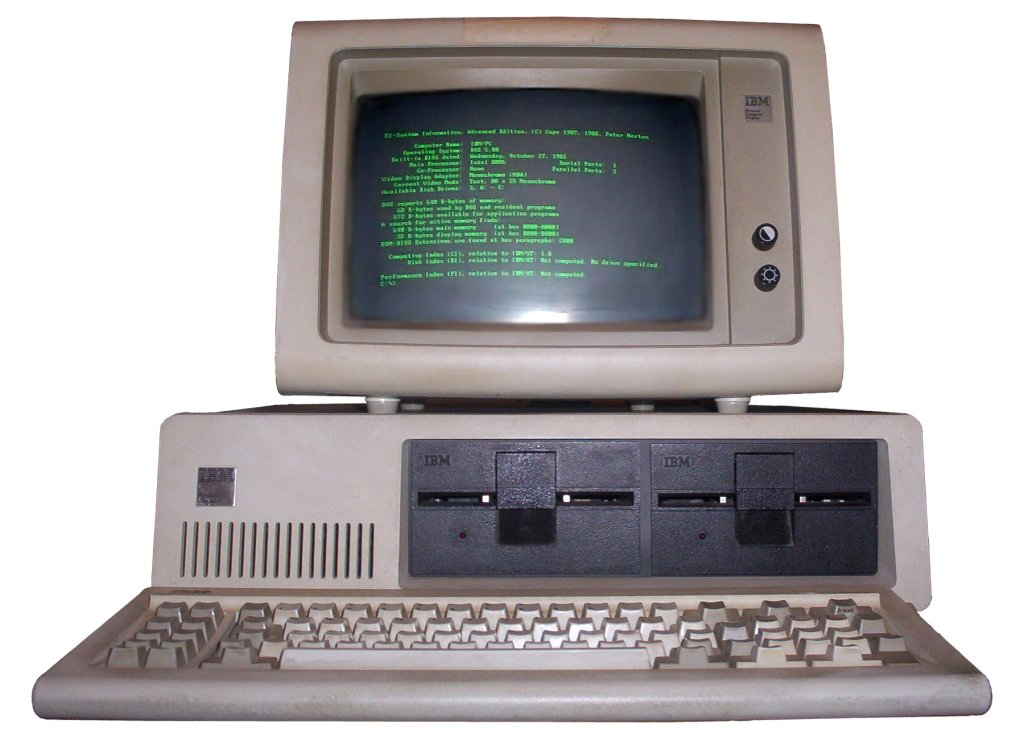
\includegraphics[width=0.5\linewidth]{img/IBM_PC_5150.jpg}
\caption{``Зелёный'' монохромный монитор с видеоадаптером MDA}
\label{ris:mda}
\end{center}
\end{figure}

В современные видеокарты встроен графический процессор, который может выполнять дополнительную обработку данных снимая тем самым нагрузку на центральный процессор. В наши дни все современные видеокарты Nvidia и AMD (Ati) выполняют обработку графических данных на аппаратном уровне.

В 1981 году был выпущен один из самых ранних графических адаптеров в истории вычислительной техники --- MDA (Monochrome Display Adapter) для компьютеров фирмы IBM PC (Рис.~\ref{ris:mda}). Данный адаптер поддерживал только текстовый режим с разрешением $80 \times 25$ символов, помимо просто текста поддерживались текстовые атрибуты: обычный, яркий, инверсный, подчёркнутый и мигающий. Какой либо графической или цветовой информации данный адаптер обрабатывать не мог, под цветностью тогда понималось лишь свечение люминофора электронно-лучевой трубки. Последующим развитием адаптера MDA стал видеоадаптер HGC (Her\-cu\-les Gra\-phics Con\-trol\-ler) созданный в 1982 году фирмой Hercules. Адаптер HGC поддерживал графическое разрешение $720 \times 348$ точек и две графические страницы. Поддержки цветов всё ещё не было.

Пионером в цветном изображении стала видеокарта CGA (Co\-lor Gra\-phics Adap\-ter) от фирмы IBM. В текстовом режиме существовало два разрешения: $40 \times 25$ символов и $80 \times 25$ символов (на каждый символ приходилась матрица $8 \times 8$ точек) с 256 символами. На каждое знакоместо приходилось 16 цветов и 16 цветов фона (либо 8 цветов фона и атрибут мигания). В графическом режиме также было два разрешения: $320 \times 200$ точек (цветность: четыре палитры по четыре цвета каждая) и $640 \times 200$ точек (данный режим был монохромным). Развитием этого адаптера стал адаптер EGA (En\-han\-ced Gra\-phics Adap\-ter) с палитрой в 64 цвета. Разрешение было увеличено до $640 \times 350$. Для режима $80 \times 25$ использовалась большая матрица --- $8 \times 14$, одновременно можно было использовать 16 цветов, цветовая палитра была расширена до 64 цветов. Графический режим также позволял использовать при разрешении $640 \times 350$ 16 цветов из палитры в 64 цвета.

В ранних моделях компьютеров от IBM PS/2 использован новый графический адаптер MCGA (Multicolor Graphics Adapter). Текстовое разрешение было поднято до $640 \times 400$, что позволило использовать режим $80 \times 50$ при матрице $8 \times 8$ точек, а для режима $80 \times 25$ использовать матрицу $8 \times 16$. Количество цветов увеличено до 262144 (64 уровня яркости по каждому цвету).


В 1987 году IBM создала компонентный видеоинтерфейс VGA (Video Graphics Array), улучшение графического адаптера MCGA. Добавлены: текстовое разрешение $720 \times 400$ для эмуляции MDA и графический режим $640 \times 480$.

В 1991 году появилось SVGA (Super VGA) --- расширение VGA с более высокими режимами и дополнительными возможностями, например, задание произвольной частоты кадров. Число цветов стало равно 65536 (High Color, 16 bit) и 16777216 (True Color, 24 bit).


\subsection{Устройство видеокарты}

На рисунке~\ref{ris:moderncard} представлен внешний вид современной видеокарты. Рассмотрим основные составные части видеокарты.

\begin{figure}[ht!]
\begin{center}
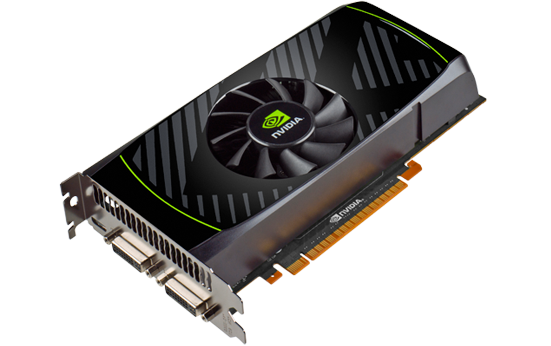
\includegraphics[width=0.5\linewidth]{img/gtx_550_ti.png}
\caption{Видеокарта NVIDIA GTX 550 TI. 2011 год.}
\label{ris:moderncard}
\end{center}
\end{figure}

\subsubsection{Графический процессор}

Графический процессор (Graphics processing unit (GPU) — графическое процессорное устройство на Рис.~\ref{ris:gpu}) часть видеокарты, занимающаяся расчётами выводимого изображения, освобождая от этой обязанности центральный процессор, производит расчёты для обработки команд трёхмерной графики. Является основой графической платы, именно от него зависят быстродействие и возможности всего устройства. Современные графические процессоры по сложности мало чем уступают центральному процессору компьютера, и зачастую превосходят его как по числу транзисторов, так и по вычислительной мощности, благодаря большому числу универсальных вычислительных блоков.

\begin{figure}[ht!]
\begin{center}
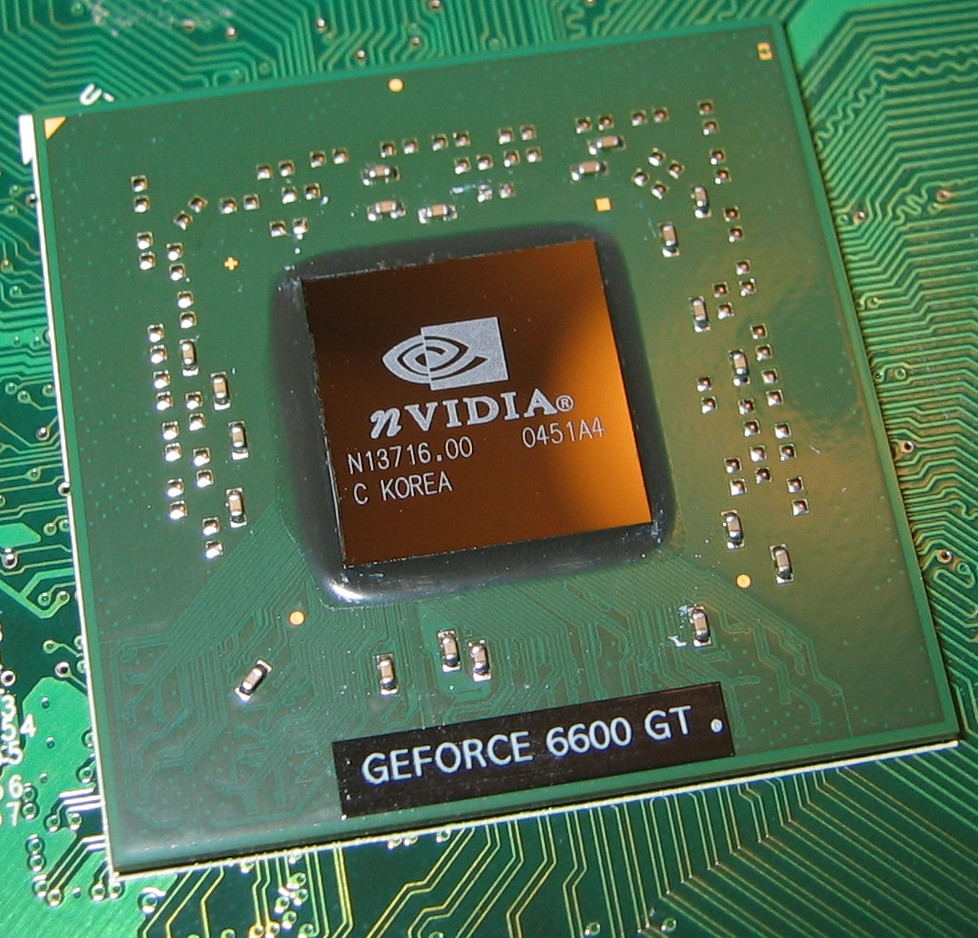
\includegraphics[width=0.3\linewidth]{img/6600GT_GPU.jpg}
\caption{Графический процессор GeForce 6600GT (NV43)}
\label{ris:gpu}
\end{center}
\end{figure}

\subsubsection{Видеоконтроллер}

Видеоконтроллер отвечает за формирование изображения в видеопамяти и осуществляет обработку запросов центрального процессора. Современные графические адаптеры (AMD, Nvidia) обычно имеют не менее двух видеоконтроллеров, работающих независимо друг от друга и управляющих одновременно одним или несколькими дисплеями каждый.

\subsubsection{Видео-ПЗУ}

Видео-ПЗУ (Video ROM) — постоянное запоминающее устройство (ПЗУ), в которое записаны BIOS видеокарты, экранные шрифты, служебные таблицы и т. п. ПЗУ не используется видеоконтроллером напрямую — к нему обращается только центральный процессор.

\subsubsection{Видео-ОЗУ}

Видеопамять выполняет функцию кадрового буфера, в котором хранится изображение, генерируемое и постоянно изменяемое графическим процессором и выводимое на экран монитора (или нескольких мониторов). В видеопамяти хранятся также промежуточные невидимые на экране элементы изображения и другие данные. Видеопамять бывает нескольких типов, различающихся по скорости доступа и рабочей частоте.

При написании истории использовался материал \cite{hist1}.
